\documentclass[runningheads,a4paper]{llncs}

%% Encoding
\usepackage[utf8]{inputenc}
\usepackage[T1]{fontenc}

%% symbols, graphics, etc
\usepackage{amssymb}
\usepackage{amsmath}
\usepackage{graphicx}
\usepackage{listings}

%% Authors and other title stuff
\title{Implementing and Solving a Contact Dynamics Problem on the GPU}
\titlerunning{Contact Dynamics on GPU}

\author{Philip Munksgaard \and Thorbjørn S. Kaiser}
\authorrunning{P. Munksgaard \and T. S. Kaiser}

\institute{
    University of Copenhagen Department of Computer Science (DIKU), \\
    Nørre Campus, Universitetsparken 5, DK-2100 Copenhagen Ø, Denmark
}

\begin{document}
\mainmatter
\maketitle

\begin{abstract}
Estimating contact impulses physical systems of rigid bodies is a
computationally expensive problem, because the impulse in each contact is a
function of all the adjacent contact impulses as well as any external
forces. In a pyramid of 2-dimensional discs, the total number of contacts is
$\frac{3h}{2} (h-1)$, and for each of these contacts we need to take up to 10
adjacent contacts into account.

We have implemented a solver for this problem that utilizes the massively
parallel architecture of GPUs in order to obtain significant performance gains
compared to a regular single-processor implementation. It turns out to be very
efficient for large pyramids with many iterations, while still leaving some
room for improvements.

\end{abstract}

\section{Introduction}

This report describes the design and implementation of a parallel Jacobi solver
for a contact dynamics problem in Haskell. The goal of this project has been to
compute the contact impulses between rigid bodies in a 2-dimensional system
using Accelerate, a Haskell embedded domain specific language (EDSL) for general
purpose GPU programming (GPGPU). To do so, and to assess the efficiency of the
parallel implementation, we also implemented the Jacobi solver, as well as a
Gauss-Seidel solver, in regular sequential Haskell.

% Thanks to Vincent and Martin?

\section{Motivation}

Simulating bodies in a system is easy, as long as no interactions between
bodies occur, eg. there are no collision. In that case, the acceleration of an
object is linearly proportional to its mass and any external forces that act
upon it. However, when rigid bodies collide there is a nonsmooth relationship
between velocities and forces that have to be handled. In complex systems with
many bodies, these collisions become very numerous, and calculating the
resulting changes in movement of the bodies become computationally expensive.

% Maybe a nice drawing of bodies flying around with no collision and then one
% with collisions?

To overcome this, we focus on computing the impulses between bodies in contact
in a given configuration of a system. Imagine a system like the one in figure
\ref{fig:pyr2simple}. It consists of three discs with unit mass and radius,
numbered from 0 to 2, in a 2-dimensional system, forming a pyramid of two
layers. Additionally there are three contacts between the bodies, named $a$,
$b$, and $c$. If there are no external forces acting upon the discs, they will
stay perfectly still and there will be no impulses. Now, imagine that we apply
a downward force to disc 0. Intuitively, we would expect that to result in an
impulse that acts upon both disc 1 and disc 2, meaning that contacts $a$ and
$b$ should have an impulse. However, we would not expect contact $c$ to have an
impulse, as discs 1 and 2 would be pushed away from each other.

\begin{figure}
  \centering
  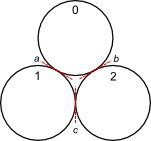
\includegraphics{figures/pyr2simple.png}
  \caption{A simple 2 layered pyramid.}
  \label{fig:pyr2simple}
  % TODO: More figures? One with a downward arrow and the resulting impulses?
\end{figure}

Naturally, the more layers we add to our pyramids, the more complex these
interactions become, as we have more contacts to take into account. For example,
in figure \ref{fig:pyr4-10}, to compute the impulse of the contact between discs
5 and 8, we have to take into accounts all the forces that act upon those two
discs. In particular, to compute the contact impulse between disc 5 and 8 we
have to take into account the contact impulses of all the disc-pairs $(2;5)$,
$(4;5)$, $(5;9)$, $(4;8)$, $(7;8)$, and $(8;9)$. Furthermore, we have to
translate the impulses in these adjacent contacts to the contact-space of the
contact between disc 5 and 8, in order to actually know what the contribution
is.

\begin{figure}
  \centering
  \includegraphics{figures/pyr4-10.png}
  \caption{A simple 4 layered pyramid, with impulses (10 iterations of Jacobi, see sections \ref{seqjacobi}, \ref{parjacobi})}
  \label{fig:pyr4-10}
\end{figure}

As can easily be imagined for this particular problem, the more layers we add,
the more contacts there are\footnote{In fact, for a height $n$, we have
  exactly $\frac{3n}{2}(n-1)$ contacts: Each layer introduces $2n-2$ contacts
  between the new layer and the old, in addition to the $n-1$ contacts in the
  new layer. We can then prove the above by induction.}, and for each contact,
we have to take up to 10 other contacts into account when calculating its
impulse, as can easily be seen in figure \ref{fig:upto10}. Furthermore, as
contact impulses depend on adjacent contact impulses, we cannot easily
calculate an analytical solution. Instead, we have to compute the solution
numerically, by using intermediate estimates to iteratively produces better and
better estimates for the contact impulses until we reach convergence.

\begin{figure}
  \centering
  \includegraphics{figures/upto10.png}
  \caption{Visualization of maximum adjacent contacts possible}
  \label{fig:upto10}
\end{figure}

Because of the massive size of these problems, and the iterative nature of the
solver, computing the contact impulses in large pyramids is expensive on
traditional sequential architectures. We wish to explore the possibility and
efficiency of computing these contact dynamics by using the data parallel
architecture of GPUs.

\section{Goals}

We wish to calculate the contact impulses between discs in a 2-dimensional
system using Accelerate, a Haskell embedded DSL for expressing parallel
computations suitable for execution on a GPU. Since transferring data to and
from the GPU can incur significant overhead, and GPU programming in general
imposes constraints on how computations can be done, we also wish to run
performance tests, comparing the GPGPU implementation with implementations of
the solver running on traditional sequential hardware, in order to discuss the
efficiency of the implementation.

\section{Contact Dynamics}

We will focus on computing the impulses for a contact $\alpha$ of a body $i$ in
one timestep. For a body $i$, let $M_i$ be the $3 \times 3$ diagonal mass
matrix, with the third component of the diagonal being the inertia of $i$, let
$V_i$ and $V_i^-$ be the velocity vectors of the current and last timestep for
the body $i$, and let $R_i$ and $R_i^{ext}$ be the external and contact impulses
applied to the body. We then have the following relationship between motion
over time for the body $i$:

\begin{equation}
  M_i(V_i - V_i^-) = R_i + R_i^{ext}
\end{equation}

Clearly, if we can find the contact impulses for the body $i$, we can find the
velocity of the body in the current step.

In order to do this, we need to find the relative velocity for each contact
between $i$ and adjacent bodies. We call a contact $\alpha$, where each
$\alpha$ has two bodies in contact, called the candiate and the antagonist. The
relative velocity $v_\alpha$ is expressed from $V_{cd}$ and $V_{an}$ as
\begin{equation}
  v_\alpha =
  \begin{pmatrix}
    H_\alpha^{cd} &
    H_\alpha^{an}
  \end{pmatrix}
  \begin{pmatrix}
    V_{cd} \\
    V_{an}
  \end{pmatrix}
\end{equation}
where $H_\alpha^{cd}$ and $H_\alpha^{an}$ are rotational matrices for the angle
between the antagonist and candidate.

For the body $i$, we may then introduce the following equation
\begin{equation}
  v_i = H_i^TV_i
\end{equation}
where $v_i$ is the concatenated vector of relative velocities for the contacts
related to $i$ and $H_i$ is the concatenated vector of rotational matrices for a
specific body and it's contacts. By duality consideration, we may also show that
the following relationship between contact impulses $r_i$ and the resultant
impulse $R_i$ on body $i$ are
\begin{equation}
R_i = H_i r_i
\end{equation}

Letting $W_i = H_i^TM_i^{-1}H_i$, we now have
\begin{align}
  & M_i(V_i - V_i^-) = R_i + R_i^{ext} \\
  \Leftrightarrow \quad & H_i^T V_i - H_i^T V_i^-) = H_i^TM_i^{-1} R_i + H_i^T
  M_i^{-1} R_i^{ext}
  \\
  \Leftrightarrow \quad & v_i - v_i^{-} = H_i^T M_i^{-1}H_i r + H_i^T M_i^{-1} R^{ext} \\
  \Leftrightarrow \quad & v_i - v_i^{-} = W_i r + H_i^T M_i^{-1} R^{ext} \\
  \Leftrightarrow \quad & W_i r - v_i = -v_i^{-} - H_i^T M_i^{-1} R^{ext}
\end{align}
Where we call $-v_i^{-} - H_i^T M_i^{-1} R^{ext}$ our right-hand side (RHS).
Additionally, for a contact $\alpha$, we have the following relationship between
its impulse $r_\alpha$ and the relative velocity of the bodies in contact
$v_\alpha$:
\begin{equation}\label{impulseXvectorConstraint}
  v_\alpha \geq 0, \quad r_\alpha \geq 0, \quad r_\alpha \cdot v_\alpha = 0
\end{equation}
Meaning that if two bodies are in contact, they are either moving away from
each other, relative to the contact normal, or they are pushing against each
other~\footnote{Additionally, there is the possibility that there is neither
  impulse nor velocity relative to the contact normal, but we can disregard
  this case, as it has no effect on the outcome}. This means, that if we can
find RHS, we can, by exclusion, find the impulse in a contact $\alpha$. For
finding the right-hand side, we use a series of continually improved estimates,
and this is where our Jacobi solver comes in.

\section{Initial Haskell implementation of the Jacobi solver\label{seqjacobi}}

The Jacobi method is an algorithm for determining the solution for a linear
system of equations. By regarding the contact impulses as our linear equations
(which makes sense since they rely on each other), the Jacobi method allows us
to iteratively refine a guess for the impulse values, until at some point they
converge.

The ordinary Haskell implementation uses the library \verb+hmatrix+, a ``purely
functional interface to basic linear algebra'', which internally uses GSL (the
GNU Scientific Library), as well as BLAS and LAPACK which are both low level
libraries for linear algebra. The entire code can be seen in appendix
\ref{app:seq}.

For each iteration of our Jacobi solver, we have to find the right-hand side of
\begin{equation} \label{lhs=rhs}
  W_{\alpha\alpha} r_\alpha^{k+1} - v_\alpha^{k+1}= - H_i^T M_i^{-1} R_i^{ext}
  - \sum\limits_{\beta \neq \alpha} W_{\alpha\beta} r_\beta^k
\end{equation}
and solve the equation with regards to the constraints given above. To do this,
we use the function \verb+iter+, which takes a list of estimated impulses, a
list of all the contacts in the system, a list of external forces for each
contact, and precomputed lists of adjacent contacts and $W_{\alpha\alpha}$
values, and runs $k$ steps of the solver.

\begin{verbatim}
iter :: (Eq a, Num a) =>
        a               -> -- Number of iterations
        [Vector Double] -> -- Previous impulses
        [Contact]       -> -- Contacts in the system
        [Vector Double] -> -- External force on each contact
        [[Int]]         -> -- List of indices for adjacent contacts
                           -- for each contact
        [Matrix Double] -> -- List of Waa for each contact a
        [Vector Double] -> -- Next impulses
iter 0 rs _ _ _ _ = rs
iter k rs cs ext adjs waas = iter (k-1) r_new cs ext adjs waas
    where
      rhss' = zipWith (sumWab cs rs) cs adjs
      rhss = zipWith (+) ext rhss'
      r_new' = zipWith solver rhss waas
      r_new = zipWith3 relaxer r_new' rs
                $ map ((1/) . fromIntegral . length) adjs
      relaxer new old relax = scale relax new + scale (1-relax) old
\end{verbatim}
Notice that we have added a relaxation term to each guess. It turned out to be
necessary in order to achieve convergence; without it, the total sum of
impulses would continue to grow forever.

The function \verb+iter+ relies on the function \verb+sumWab+ which takes a
contact and sums up the products of adjacent contacts and their impulses.
\begin{verbatim}
sumWab :: [Contact] -> [Vector Double] -> Contact -> [Int] -> Vector Double
sumWab cs rs c adjs =
    neg $ foldr add (fromList [0, 0]) prods
        where
          prods = zipWith mXv wabs $ pick rs adjs
          wabs = map (wab c) $ pick cs adjs
\end{verbatim}

Finally, we need the function \verb+solver+, to actually compute the new
impulse for a contact given the right hand side.
\begin{verbatim}
solver :: (Ord a, Field a) => Vector a -> Matrix a -> Vector a
solver rhs waa =
    if (rhs @> 0) > 0 then
        inv waa `mXv` rhs
    else
        fromList [0, 0]
\end{verbatim}

All in all, these functions allow us to iteratively estimate the contact
impulses for a set of discs.

\subsection{The Gauss-Seidel solver}

We have also implemented a solver using the Gauss-Seidel method, which, while
very similiar to the Jacobi method in its basic outline, is conceptually
different, and yields slightly different results for our tests.

Where the solver using the Jacobi method does a complete run through all the
contacts in a configuration before they are updated, the Gauss-Seidel solver
updates the impulse estimates after each contact has been processed. So in
effect, while the Jacobi metod allows for contact impulse estimates to be
computed in parallel in each iteration, the contact impulse values computed
with the Gauss-Seidel method depends on the contact impulse values for all the
previous contact impulse values found \emph{in that same iteration}.

To compute contact impulses using the Gauss-Seidel method, we use the following
two functions, in addition the some of the helper functions from before:
\begin{verbatim}
gauss :: Int -> [Disc] -> [Vector Double] -> [Vector Double]
gauss n ds ext' =
  gauss' n r_init
    where
      cs = contacts ds
      ncs = length cs - 1
      adjs = zipWith (`adjContacts` cs) cs (iterate (+ 1) 0)
      waas = map waa cs
      r_init = replicate (length cs) $ fromList [0, 0]
      ext = zipWith calcExt ext' cs
      gauss' 0 rs = rs
      gauss' n rs = gauss' (n-1) $
                    iter' ncs rs cs ext adjs waas
\end{verbatim}
\begin{verbatim}
iter' (-1) rs _ _ _ _ = rs
iter' i rs cs ext adjs waas  =
    iter' (i-1) (set i new_r rs) cs ext adjs waas
      where
        new_r = solver rhs waa
        waa = waas !! i
        rhs' = sumWab cs rs (cs !! i) (adjs !! i)
        rhs = if i < 2 then
                ext !! i + rhs'
              else
                rhs'
\end{verbatim}
Apart from the difference in method, we don't apply relaxation when using the
Gauss-Seidel model, which might also explain why our results never converge to
a single value. Instead, after a number of iterations, the Gauss-Seidel method
seems to settle on a handful of different configurations, which it then cycles
between. This is to be expected, given the nature of the Gauss-Seidel
method. However, it is very possible that some form of relaxation could help
alleviate that problem.

\section{Parallel implementation in Accelerate\label{parjacobi}}
Porting code from a conventional single-CPU architecture to the massively
parallel SIMD architecture of GPUs, is, in general, not trivial. The SIMD
architecture imposes many constraints on how effectively certain computations
can be performed. For example, branches in the code, such as \verb+if+
statements or the like, have to be sequentialized in order to run on the
GPU. That is, if an \verb+if+ statement introduces two new ``branches'' in the
code, the GPU cannot compute the two branches in parallel, but must instead
compute the first branch by itself, followed by the second branch. Similarly,
GPUs cannot handle arbitrary data types such as nested data structures
(eg. arrays in arrays) or functional values. However, GPUs excel at performing
lots of identical but independent computations across large arrays or
matrices. For example, adding two large matrices together is trivially
parallelizable, since each core on the GPU can add indices from the matrices
together, independently from all the other cores. When porting code to the GPU,
it is therefore imperative that we have these limitations and advantages in
mind.

Accelerate allows us to express computations for the GPU inside
Haskell. However, in order to do so without sacrificing too much of the speed
advantage that GPUs enable, it imposes even further restrictions on what we can
express. First of all, we have to explicitly move data back and forth between
the host and the GPU, but secondly the language for expressing computations on
the GPU is rather limited. Most importantly, we can only use flat
data-parallelism involving only regular, multi-dimensional arrays; Accelerate
is a stratified language, which distinguishes between collective and scalar
computations.

\subsection{Identifying parallel structure in sequential code\label{identpara}}
Looking at the sequential implementation
of the Jacobi solver
we can immediately see avenues for gainful parallelization.
Calculating and solving the impulses
for each iteration is independent between each contact,
as the only dynamic data is the impulses,
for which we only look at the previous iteration's results.
So logically the iterations have to be sequential,
while the calculations of the next impulses in an iteration
can be done in parallel.

This is in contrast to the sequential Gauss-Seidel implementation
where solving the impulse for a contact depends
on the results from solving the previous contacts impulses
in the same iteration.
The naive Gauss-Seidel implementation,
while gainful in the sequential case,
enforces a sequential structure on the execution
and is thus hard to parallelize\footnote{
  Although maybe not impossible. A possibility not explored by us
  would be to graph the relationships between the contacts
  and cut the graph such that we parallelize the calculations
  of contacts which do not depend on each other.
  Thus solving a given cut would be parallel,
  but solving all the cuts would still be sequential.
  If the graph is sparse, the number of cuts could be very low.}.

Another place we can parallelize is the calculation
of the matrix-vector product sums in \eqref{lhs=rhs},
that is \[\sum\limits_{\beta \neq \alpha} W_{\alpha\beta} r_\beta^k\]
as each component of the sum is independent from the next,
and the summing itself is trivially commutative,
so nothing stops us from calculating each component in parallel
and then folding the results in parallel.

And lastly solving each right hand side of \eqref{lhs=rhs}
to get the next impulses can also trivially be done in parallel.

\subsection{Solving the right hand sides}
In explaining our parallel implementation we will start
by going backwards, first explaining the solving,
then the calculating of the right hand side in general,
and finally calculating the matrix-vector product sums specifically.

The code for the Accelerate solver is as follows
\begin{verbatim}
solveRHS :: Acc (VectorList Double) -> 
            Acc (VectorList Double) -> 
            Acc (VectorList Double)
solveRHS inWaas rhss = A.zipWith (*) condM 
                     $ A.zipWith (*) inWaas rhss
  where
    condM   = A.replicate repSh 
            $ A.map (A.fromIntegral . boolToInt . (>*0)) rhs1s
    rhs1s   = slice rhss sliceSh
    sliceSh = lift $ Z :.All :.i0
    repSh   = lift $ Z :.All :.i2
\end{verbatim}
here \texttt{rhss} is the right hand side for each contact,
and \texttt{inWaas} is the inverse of $W_{\alpha\alpha}$ for each contact.

We have to solve the problem of \eqref{impulseXvectorConstraint}:
we wish to see whether the velocity is positive,
which it is iff the right hand side is negative.
We only test the first component of the RHS
as we do not handle friction in the model and is thus only interested
in the component out of the contact normal ie. the first component.

Instead of testing as we solve,
which would lead to SIMD divergence due to how the GPU handles branching,
we solve for all rhss in parallel and then filter out the results
using a conditional matrix.

\subsection{Calculating the right hand sides}
The code for the Accelerate RHS calculator is as follows
\begin{verbatim}
           -- number of contacts, used for replication in wXr
calcRHS :: Exp Int                 ->
           -- external forces (negated form)
           Acc (VectorList Double) ->
           -- NxNx2x2 matrix holding Wabs for each contact
           Acc Wxxss               ->
           -- previous impulses for each contact
           Acc (VectorList Double) ->
           -- right hand sides
           Acc (VectorList Double) ->
calcRHS n extF wabss rs = extF `vssub` (wabss `wXr'` rs)
  where
    wXr'  = wXr n
\end{verbatim}

The array \texttt{wabss} bears some explaining.
As we wish to calculate the RHS for each contact at the same time,
and also wish to parallelize calculating the matrix-vector product sums,
we run into nested data parallelism in the naive implementation,
which Accelerate does not support.

So to summarize: we have two loops, one nested in the other, that we wish to parallelize
\begin{enumerate}
\item Calculating RHS for each contact
\item Calculating the matrix vector product for each $W_{\alpha\beta} \cdot r_{\beta}$ and summing them
\end{enumerate}

To flatten the nested data parallelism we resort to work in higher dimensions,
with the extra dimensions conceptually encoding the two loops.
Thus \texttt{wabss} is an $n \times n \times 2 \times 2$ array,
with $n$ being the number of contacts.
The two inner ($2 \times 2$) dimensions can thus be viewed
as the elements of a $n \times n$ array,
where the rows are the contacts $\alpha$,
the columns are the adjacent contacts $\beta$,
and the elements are the individual $W_{\alpha\beta}$.
It should be noted that in the case where two contacts are not adjacent
the $W_{\alpha\beta}$ is the null matrix.

With this explained the semantics of the code follows \eqref{lhs=rhs} closely.

\subsection{Calculating the matrix-vector product sums}
In the function for \texttt{calcRHS} we did the matrix-vector product sums
for all the contacts at the same time using the \texttt{wXr} function.
The code for it is as follows
\begin{verbatim}
wXr :: Exp Int ->
       Acc Wxxss ->
       Acc(VectorList Double) ->
       Acc(VectorList Double)
wXr n wabss rs' = rowRowSums
  where
    rowRowSums = permute (+) zeros rowFold products
    products   = A.zipWith (*) wabss rs
    zeros      = fill nx2Sh d0
    rs         = A.replicate repSh2 $ A.replicate repSh1 rs'
    nx2Sh      = lift $ Z :.n   :.i2
    repSh2     = lift $ Z :.n   :.All :.All :.All
    repSh1     = lift $ Z :.All :.i2  :.All
    rowFold ix = index2
                 (indexHead $ indexTail $ indexTail $ indexTail ix)
                 (indexHead $ indexTail ix)
\end{verbatim}

\texttt{wabss} is on the form explained in the previous section.
What we want to do is for each row and for each $W_{\alpha\beta}$
do matrix-vector multiplication with their respective $r_\beta$
and then fold.

Trivially the matrix-vector multiplication is of the form
\[
W_{\alpha\beta} \cdot r_\beta = 
\begin{pmatrix}
W_{1,1} \cdot r_{1} + W_{1,2} \cdot r_{2} \\
W_{2,1} \cdot r_{1} + W_{1,2} \cdot r_{2}
\end{pmatrix}
\]
for each element.
To do this in parallel for all $W_{\alpha\beta}$s
we first replicate the components of \texttt{rs'}
into a new dimension so that we get a new $n \times 2 \times 2$
array that can be seen as a $n$ length vector with $2 \times 2$
arrays as elements of the form
\[
\begin{bmatrix}
r_{1} & r_{2} \\
r_{1} & r_{2}
\end{bmatrix}
\]

and we then replicate again, across a new row dimension,
$n$ times such that we end up with an $n \times n \times 2 \times 2$
where we can do elementwise multiplication with \texttt{wabss} in parallel.

After this multiplication step of the elements we then do the remaining addition and summation
via a permutation into an $n \times 2$ array, yielding the final matrix-vector product sums
for each contact.

\subsection{Relaxation}
Finally we do the relaxation step outside in the iterator itself,
\begin{verbatim}
iter :: Int ->
        Acc (VectorList Double) ->
        (Acc (VectorList Double) -> Acc (VectorList Double)) ->
        Acc (VectorList Double) ->
        Acc (VectorList Double)
iter 0 _ _ rs = rs
iter n w solver rs = iter (n-1) w solver rs''
  where
    rs'' = A.zipWith (+)
           (A.zipWith (*) w rs')
           (A.zipWith(\x y -> (1-x) * y) w rs)
    rs'  = solver rs
\end{verbatim}
where $w$ is the relaxation variables for each contact,
as described in the sequential solver,
and the solver is the Accelerate solver initialized
with all the relevant data.

\subsection{Construction and lifting of data\label{dataconstruction}}
When implementing the parallel solution
we focused on the iteration step itself
and lifted all calculations of static data
outside of the solver.
This include precalculating the following values,
sequentially, as they do not change between the steps

\begin{itemize}
\item All contacts were found
\item $W_{\alpha\alpha}$ was calculated and the inverses found
\item Adjacency was calculated, including all the $W_{\alpha\beta}$ matrices
\item Relaxation parameter $w$ was calculated
\end{itemize}

The calculation of these values are included in the overhead for both
the sequential and parallel implementations,
where the parallel solution calculates it all in the host memory
before lifting the results into the device memory.

Further speed increases could possibly be gained
by also looking at parallelization of the collision detection
and the calculation of all these static values,
but we intentionally left it out as we focused on the algorithm
for calculating the iterations.

\section{Results}

\section{Future Work}
During the course of implementing our solution and writing this
paper we left out exploring some optimizations that we feel
might be worthwhile to do, as we focused on parallelizing
the core iteration step of the Jacobi solver.

\begin{itemize}
\item As described in section \ref{dataconstruction} we left out
  parallelizing the precalculation of the static data.
  Especially the collision and adjacency detection could be worthwhile
  to do in parallel, both as it lends itself to parallelization
  and because it cuts down on the amount of data to send to the device.
\item Find and implement parallel structure in the code for the Gauss-Seidel iteration.
  Inherently this method is sequential, but as we noted in section \ref{identpara}
  there could be methods such as graph cutting of the adjacency graph
  that could lead to independent parts of the iteration to be calculated in parallel.
\item Implement calculating the velocity changes for the discs based
  on the results of the iteration, as well as look at how many iterations are needed
  for reasonably accurate results across multiple time steps.
\item Implement a solution in 3 dimensions, instead of only 2.
  This should be reasonably straight-forward, as the algorithm is the same
  but with more dimensions, but making it fast might be a challenge.
\item Implement handling of friction and rotation of the discs.
\end{itemize}

\section{Conclusion}

We have implemented three different methods for calculating the contact
impulses between rigid bodies in a 2-dimensional system. First we used Haskel
to create a Jacobi solver, then we slightly modified the Jacobi solver in order
to obtain a Gauss-Seidel solver, and finally we implemented the a parallelized
Jacobi solver using Accelerate, which targets the GPU.

By utilizing the GPUs massively parallel architecture for our Jacobi solver, we
obtained significant performance gains. And while there are avenues
for improving the sequential solvers, so is the case for the parallel solver,
where we expect to see even greater performance gains.

\begin{thebibliography}{4}
\bibitem{proceeding2} Chakravarty, Manuel MT, et al.: ``Accelerating Haskell
  array codes with multicore GPUs.'' Proceedings of the sixth workshop on
  Declarative aspects of multicore programming. ACM, (2011).

\bibitem{proceeding2} Keller, Gabriele, et al.: ``Regular, shape-polymorphic,
  parallel arrays in Haskell.'' ACM Sigplan Notices. Vol. 45. No. 9. ACM, 2010.
\end{thebibliography}

\end{document}
